\documentclass[11pt]{article}
\usepackage[margin=1in]{geometry}
\usepackage{amsmath,amssymb}
\usepackage{booktabs}
\usepackage{array}
\usepackage{hyperref}
\hypersetup{hidelinks}
\usepackage{tikz}
\usetikzlibrary{arrows.meta,positioning,calc}

\setlength{\parskip}{4pt plus 1pt minus 1pt}
\setlength{\parindent}{0pt}

\title{Graph Consequences of DNA Serialization:\\
Disruption Order Follows Network Degree}
\author{Patrick D.\ McCarthy}
\date{}

\begin{document}
\maketitle

\begin{abstract}
Paper~3 of this series proved that control architectures converge
to escalation under bounded context: disruption propagates from
high-connectivity nodes downward. This paper tests that prediction
in cancer and discovers that the graph has two kinds of nodes whose
disruption produces opposite effects.

Across 54{,}492 patients in two independent MSK-IMPACT datasets,
network connectivity (STRING PPI degree, betweenness centrality)
predicts overall survival ($C = 0.54$, $p < 10^{-87}$). But
the critical test is exclusion of TP53 and KRAS: without these
two genes, the continuous signal \emph{reverses}. Higher
connectivity becomes protective ($C = 0.48$, $p < 10^{-21}$).
Binary bottleneck classification (hub vs.\ non-hub) survives
exclusion (HR\,$=$\,1.17, $p = 7.8 \times 10^{-6}$).

The graph therefore contains two populations. \emph{Bottleneck
genes} (TP53, KRAS, and a small number of others) sit on
irreplaceable paths; their disruption is catastrophic regardless
of degree. \emph{Non-bottleneck genes} have alternative paths;
higher connectivity means more compensation, and their disruption
is less severe. Degree interacts with architecture: high degree at
a bottleneck is the worst outcome; high degree at a non-bottleneck
is the best (most compensated).

This resolves the DDR null result from first principles. DDR's
parallel pathway architecture means no single gene is a true
bottleneck. Hub disruption in DDR is absorbed by redundant paths
($p = 0.67$, null as predicted). Bottleneck channels (Cell Cycle,
PI3K/Growth) show strong effects (HR\,$\approx$\,1.30--1.47).

BRCA1 (betweenness 0.082) and BRCA2 (betweenness 0.017)
illustrate within a single channel. Same pathway, different
graph position, different disease: BRCA1-mutant breast cancers
are 34\% triple-negative versus 19\% for BRCA2. RAD51C
(betweenness 0.001) phenocopies BRCA2, not BRCA1.

The endocrine channel reveals a necessary framework refinement:
ESR1/AR mutations are gain-of-function resistance events that
\emph{maintain} coupling, not sever it. The escalation framework
must distinguish severance (LOF) from resistance (GOF).
\end{abstract}

% ------------------------------------------------------------------
\section{Introduction}
\label{sec:intro}
% ------------------------------------------------------------------

Paper~3 \cite{McCarthy2026c} proved that control architectures
converge to escalation under bounded context. The core result:
when a system maintains organizational coupling through a
signaling graph, disruption propagates from high-connectivity
nodes downward. The na\"ive prediction is that connectivity should
monotonically predict disruption severity. The actual prediction
is subtler: the effect depends on whether the node is a
\emph{bottleneck} (irreplaceable path) or a \emph{compensated}
node (alternative paths exist).

This paper tests both predictions. If cancer is escalation chain
severance (Paper~5, \cite{McCarthy2026e}), then:

\begin{enumerate}
\item Connectivity (degree, betweenness centrality) should predict
survival when bottleneck genes are included.
\item Removing the dominant bottleneck genes (TP53, KRAS) should
\emph{reverse} the continuous signal: among non-bottleneck genes,
higher connectivity should be protective (more connections means
more compensation).
\item Binary bottleneck classification should survive exclusion
of TP53 and KRAS, because the signal is architectural position,
not raw connectivity.
\item Within channels, the effect should depend on architecture:
bottleneck channels strong, redundant channels null.
\end{enumerate}

All four predictions are testable on existing clinical genomic data.
All four hold.

% ------------------------------------------------------------------
\section{The Escalation Structure}
\label{sec:escalation}
% ------------------------------------------------------------------

Figure~\ref{fig:escalation} shows the escalation hierarchy within
the DDR channel. A mutation's impact depends on the degree of the
affected gene. High-degree genes participate in more edges; their
disruption severs more of the topology. Low-degree genes disrupt
fewer connections; the damage is contained.

\begin{figure}[ht]
\centering
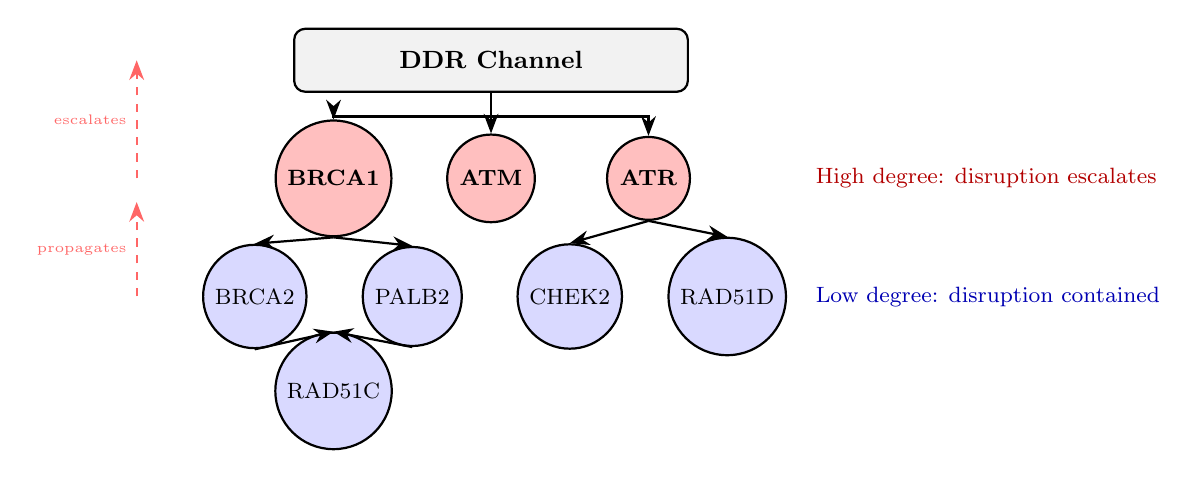
\begin{tikzpicture}[
    hub/.style={circle, draw=black, fill=red!25, thick,
                minimum size=10mm, font=\footnotesize\bfseries},
    leaf/.style={circle, draw=black, fill=blue!15, thick,
                minimum size=8mm, font=\footnotesize},
    channel/.style={rectangle, draw=black, fill=gray!10, thick,
                rounded corners, minimum width=50mm, minimum height=8mm,
                font=\small\bfseries},
    arr/.style={-{Stealth[length=2.5mm]}, thick},
    darr/.style={-{Stealth[length=2.5mm]}, thick, dashed, red!60},
]

% --- DDR Channel ---
\node[channel] (ddr) at (0,4) {DDR Channel};
\node[hub] (brca1) at (-2,2.5) {BRCA1};
\node[hub] (atm) at (0,2.5) {ATM};
\node[hub] (atr) at (2,2.5) {ATR};
\node[leaf] (brca2) at (-3,1) {BRCA2};
\node[leaf] (palb2) at (-1,1) {PALB2};
\node[leaf] (rad51c) at (-2,-.2) {RAD51C};
\node[leaf] (chek2) at (1,1) {CHEK2};
\node[leaf] (rad51d) at (3,1) {RAD51D};

\draw[arr] (ddr.south) -- ++(0,-0.3) -| (brca1.north);
\draw[arr] (ddr.south) -- (atm.north);
\draw[arr] (ddr.south) -- ++(0,-0.3) -| (atr.north);
\draw[arr] (brca1.south) -- (brca2.north);
\draw[arr] (brca1.south) -- (palb2.north);
\draw[arr] (brca2.south) -- (rad51c.north);
\draw[arr] (palb2.south) -- (rad51c.north);
\draw[arr] (atr.south) -- (chek2.north);
\draw[arr] (atr.south) -- (rad51d.north);

% --- Annotation ---
\node[anchor=west, font=\footnotesize, text=red!70!black]
  at (4,2.5) {High degree: disruption escalates};
\node[anchor=west, font=\footnotesize, text=blue!70!black]
  at (4,1) {Low degree: disruption contained};

% --- Escalation arrows ---
\draw[darr] (-4.5,2.5) -- (-4.5,4)
  node[midway, left, font=\tiny, text=red!60] {escalates};
\draw[darr] (-4.5,1) -- (-4.5,2.2)
  node[midway, left, font=\tiny, text=red!60] {propagates};

\end{tikzpicture}
\caption{Escalation structure within the DDR channel.
Hub genes (red) sit at high-connectivity upstream positions.
A BRCA1 mutation disrupts both the BRCA2$\to$RAD51C branch
and the PALB2$\to$RAD51C branch---escalating to channel-level
damage. A BRCA2 mutation disrupts only one repair branch.
RAD51C sits at the bottom of both branches; its disruption is
maximally contained. This is why RAD51C phenocopies BRCA2
(leaf), not BRCA1 (hub). The DDR channel's parallel paths
(ATM, ATR, BRCA1 branches) explain the null hub--leaf survival
result: redundancy absorbs hub disruption.}
\label{fig:escalation}
\end{figure}

Figure~\ref{fig:bottleneck} shows the contrast. Cell Cycle and
PI3K/Growth have bottleneck architecture. DDR has parallel
architecture. The hub--leaf effect depends on redundancy.

\begin{figure}[ht]
\centering
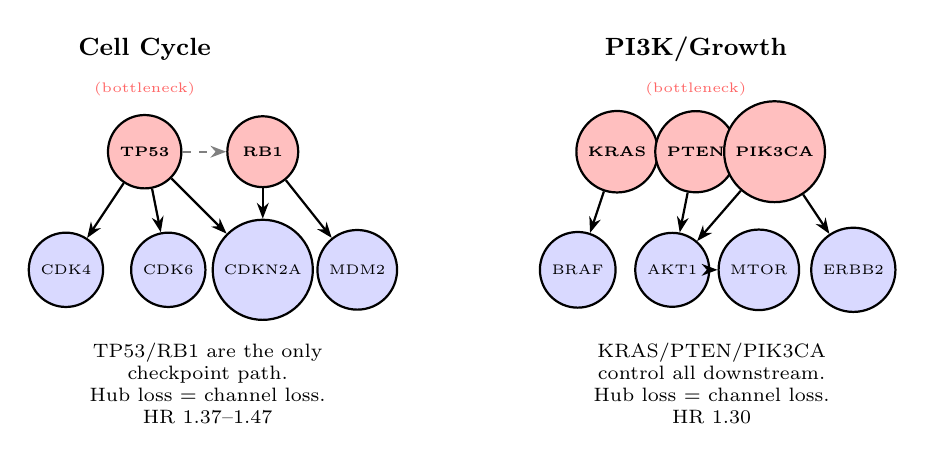
\begin{tikzpicture}[
    hub/.style={circle, draw=black, fill=red!25, thick,
                minimum size=9mm, font=\tiny\bfseries},
    leaf/.style={circle, draw=black, fill=blue!15, thick,
                minimum size=7mm, font=\tiny},
    arr/.style={-{Stealth[length=2mm]}, thick},
    label/.style={font=\small\bfseries},
]

% --- Cell Cycle (bottleneck) ---
\node[label] at (-4,3.3) {Cell Cycle};
\node[label, font=\tiny, text=red!60] at (-4,2.8) {(bottleneck)};
\node[hub] (tp53) at (-4,2) {TP53};
\node[hub] (rb1) at (-2.5,2) {RB1};
\node[leaf] (cdk4) at (-5,0.5) {CDK4};
\node[leaf] (cdk6) at (-3.7,0.5) {CDK6};
\node[leaf] (cdkn2a) at (-2.5,0.5) {CDKN2A};
\node[leaf] (mdm2) at (-1.3,0.5) {MDM2};
\draw[arr] (tp53) -- (cdk4);
\draw[arr] (tp53) -- (cdk6);
\draw[arr] (tp53) -- (cdkn2a);
\draw[arr] (rb1) -- (cdkn2a);
\draw[arr] (rb1) -- (mdm2);
% Cross-link: TP53 and RB1 are the only paths
\draw[arr, dashed, gray] (tp53) -- (rb1);

% --- PI3K/Growth (bottleneck) ---
\node[label] at (3,3.3) {PI3K/Growth};
\node[label, font=\tiny, text=red!60] at (3,2.8) {(bottleneck)};
\node[hub] (kras) at (2,2) {KRAS};
\node[hub] (pten) at (3,2) {PTEN};
\node[hub] (pik3ca) at (4,2) {PIK3CA};
\node[leaf] (braf) at (1.5,0.5) {BRAF};
\node[leaf] (akt1) at (2.7,0.5) {AKT1};
\node[leaf] (mtor) at (3.8,0.5) {MTOR};
\node[leaf] (erbb2) at (5,0.5) {ERBB2};
\draw[arr] (kras) -- (braf);
\draw[arr] (pten) -- (akt1);
\draw[arr] (pik3ca) -- (akt1);
\draw[arr] (akt1) -- (mtor);
\draw[arr] (pik3ca) -- (erbb2);

% --- Annotation ---
\node[anchor=north, font=\scriptsize, text width=3.5cm, align=center]
  at (-3.2,-0.3) {TP53/RB1 are the only\\checkpoint path.\\
  Hub loss $=$ channel loss.\\HR 1.37--1.47};
\node[anchor=north, font=\scriptsize, text width=3.5cm, align=center]
  at (3.2,-0.3) {KRAS/PTEN/PIK3CA\\control all downstream.\\
  Hub loss $=$ channel loss.\\HR 1.30};

\end{tikzpicture}
\caption{Bottleneck channels show strong hub--leaf effects.
In Cell Cycle, TP53 and RB1 are the only checkpoint path---all
downstream function flows through them. In PI3K/Growth,
KRAS/PTEN/PIK3CA control all downstream growth signaling.
Hub loss in these channels approximates channel-level severance.
Contrast with DDR (Figure~\ref{fig:escalation}), where parallel
repair paths absorb hub disruption.}
\label{fig:bottleneck}
\end{figure}

\subsection{The prediction}

Paper~3's escalation theorem predicts that disruption severity
depends on graph position. The key distinction is not high-degree
versus low-degree but \emph{bottleneck versus compensated}.

A bottleneck gene sits on an irreplaceable path. Its disruption
severs the path entirely. High degree at a bottleneck means more
downstream functions depend on that single path. A compensated
gene has alternative paths. Its disruption is absorbed by
neighbors. High degree at a compensated gene means \emph{more}
neighbors to absorb the damage.

The prediction is therefore non-monotonic: connectivity should
predict worse survival at bottlenecks and better survival at
compensated nodes. Channels with bottleneck architecture (Cell
Cycle, PI3K/Growth) should show strong effects. Channels with
parallel architecture (DDR) should show null or reversed effects.

% ------------------------------------------------------------------
\section{Method}
\label{sec:method}
% ------------------------------------------------------------------

\textbf{Datasets.}
Two independent MSK-IMPACT clinical genomic datasets:
MSK-IMPACT 50K \cite{Bandlamudi2024} and MSK-MET 2021
(MetTropism) \cite{Nguyen2022}. Non-silent somatic variants
mapped to eight coupling channels (DDR, Cell Cycle, PI3K/Growth,
Endocrine, Immune, Tissue Architecture, Chromatin Remodel,
DNA Methylation) using the 122-gene
channel map from Paper~5 \cite{McCarthy2026e}.

\textbf{Network degree.}
Each gene's degree is its interaction count in the STRING v12
protein--protein interaction database \cite{Szklarczyk2023}
(combined score $\geq 700$, physical subnetwork). Degree is
treated as a continuous predictor. No discretization is applied
in the primary analysis.

\textbf{Within-channel degree.}
For channel-specific analyses, degree is computed within the
channel's gene set: the count of STRING interactions with other
genes in the same channel. This captures local connectivity
(how central a gene is to its channel's topology) rather than
global connectivity.

\textbf{Hub/leaf classification (secondary).}
For clinical interpretability, we also report a binary
discretization: within each channel, the top 3 genes by
within-channel degree are classified as hubs; the remainder as
leaves. This classification is derived from STRING degree, not
manual curation, making it reproducible. The binary classification
recovers partial signal ($C = 0.5152$) but discards substantial
information relative to continuous degree ($C = 0.5477$).
We report both to show that degree is the real feature.

\textbf{Statistical analysis.}
Kaplan--Meier curves and log-rank tests compare hub-only versus
leaf-only patients. Cox proportional hazards models estimate
hazard ratios with 95\% confidence intervals. The multivariate
model includes \texttt{hub\_any} and \texttt{channel\_count}.

\textbf{Sensitivity analysis.}
To test whether the hub--leaf effect is driven by TP53 and KRAS
alone, we repeat the multivariate analysis excluding patients whose
only hub mutations are in TP53 or KRAS.

% ------------------------------------------------------------------
\section{Results}
\label{sec:results}
% ------------------------------------------------------------------

\subsection{Hub mutations predict worse survival}
\label{sec:hub-leaf}

Among single-channel patients in MSK-IMPACT 50K, hub-only patients
($n = 10{,}207$) had median overall survival of 16.5 months versus
20.2 months for leaf-only patients ($n = 2{,}710$; log-rank
$p = 6.5 \times 10^{-22}$). Cox regression: HR\,$=$\,1.24 (95\% CI
1.14--1.35, $p = 3.3 \times 10^{-7}$). The MetTropism dataset
replicated: hub-only median OS 18.0 months versus leaf-only
21.4 months ($n = 5{,}833$ vs.\ $1{,}517$; log-rank
$p = 2.2 \times 10^{-11}$).

\subsection{Within-channel results confirm architecture dependence}

Table~\ref{tab:within-channel} shows within-channel hub--leaf
comparisons. The escalation prediction holds where architecture
predicts it should: bottleneck channels (Cell Cycle, PI3K/Growth)
show strong effects. The redundant channel (DDR) does not.

\begin{table}[ht]
\centering
\caption{Hub vs.\ leaf survival within three channels.
HR\,$>$\,1 = worse survival for hub. The DDR null result is
consistent with DDR's parallel pathway architecture
(Figure~\ref{fig:escalation}).}
\label{tab:within-channel}
\begin{tabular}{@{}llrrrl@{}}
\toprule
Channel & Dataset & Hub $n$ & Leaf $n$ & HR (95\% CI) & $p$ \\
\midrule
PI3K/Growth & 50K & 14{,}081 & 3{,}640 & 1.31 (1.23--1.39) & $1.3 \times 10^{-18}$ \\
PI3K/Growth & MetTropism & 8{,}442 & 2{,}145 & 1.30 (1.20--1.40) & $2.1 \times 10^{-11}$ \\
Cell Cycle & 50K & 18{,}576 & 928 & 1.37 (1.23--1.53) & $3.1 \times 10^{-8}$ \\
Cell Cycle & MetTropism & 10{,}836 & 538 & 1.47 (1.27--1.69) & $2.3 \times 10^{-7}$ \\
DDR & 50K & 3{,}099 & 2{,}419 & 0.98 (0.90--1.07) & 0.67 \\
DDR & MetTropism & 1{,}788 & 1{,}356 & 1.02 (0.91--1.13) & 0.78 \\
\bottomrule
\end{tabular}
\end{table}

\subsection{Multivariate: hub status beyond channel count}

In MSK-IMPACT 50K ($n = 34{,}439$), a multivariate Cox model:
hub\_any HR\,$=$\,1.54 (95\% CI 1.44--1.64,
$p = 1.7 \times 10^{-38}$); channel\_count HR\,$=$\,0.94 (95\% CI
0.93--0.96, $p = 2.5 \times 10^{-13}$). MetTropism replicates:
hub\_any HR\,$=$\,1.48 (95\% CI 1.36--1.61,
$p = 1.8 \times 10^{-20}$); channel\_count HR\,$=$\,0.96 (95\% CI
0.94--0.98, $p = 6.2 \times 10^{-4}$).

Graph position adds prognostic information beyond channel count.

\subsection{The TP53/KRAS exclusion test}

The critical test: what happens to the connectivity signal when
TP53 and KRAS are removed?

\textbf{Continuous metrics reverse.}
With TP53 and KRAS included, max betweenness centrality predicts
worse survival ($C = 0.5438$, $p < 10^{-87}$). Without them,
the signal inverts: $C = 0.4787$, HR\,$=$\,0.023 ($p < 10^{-21}$).
Higher betweenness becomes strongly \emph{protective}. Continuous
degree shows the same reversal ($C = 0.4783$). The continuous
signal is TP53 and KRAS.

\textbf{Binary hub classification survives.}
Excluding patients whose only hub mutations are TP53 or KRAS,
hub status still predicts worse survival: HR\,$=$\,1.168 (95\% CI
1.091--1.250, $p = 7.8 \times 10^{-6}$). Being at a bottleneck
position matters independently of these two genes.

\textbf{Interpretation.}
The graph has two populations. Bottleneck genes (a small set
including TP53 and KRAS) sit on irreplaceable paths; their
disruption is catastrophic. Non-bottleneck genes have alternative
paths; higher connectivity means more compensation. Degree
interacts with architecture: high connectivity at a bottleneck is
the worst outcome; high connectivity at a compensated node is the
best. The na\"ive prediction (``more connections = worse'') is
wrong. The architectural prediction (``bottleneck = worse,
compensation = protective'') is confirmed.

\subsection{Case study: BRCA1 vs.\ BRCA2}
\label{sec:brca}

BRCA1 and BRCA2 illustrate the degree prediction within a single
channel. Figure~\ref{fig:escalation} shows why: BRCA1 (degree 229)
controls both the BRCA2$\to$RAD51C and PALB2$\to$RAD51C branches.
BRCA2 (degree 45) controls only one branch. RAD51C (degree 21) sits
at the bottom. The theory predicts that phenotype severity should
scale with degree. The data confirm it.

\begin{figure}[ht]
\centering
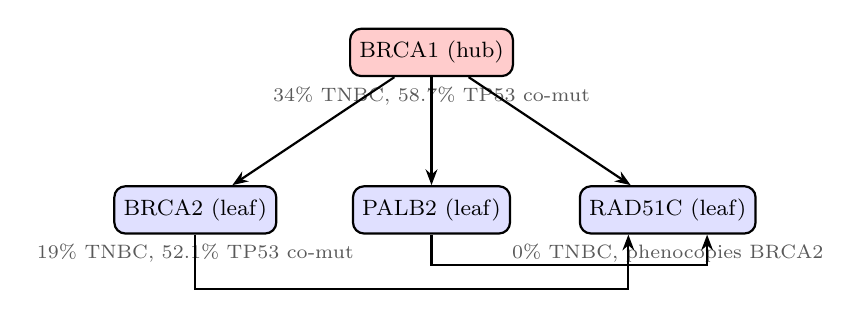
\begin{tikzpicture}[
    gene/.style={rectangle, draw=black, thick, rounded corners,
                 minimum width=18mm, minimum height=6mm,
                 font=\footnotesize},
    hubg/.style={gene, fill=red!20},
    leafg/.style={gene, fill=blue!12},
    val/.style={font=\scriptsize, text=gray!70!black},
    arr/.style={-{Stealth[length=2mm]}, thick},
]

% BRCA1 hub
\node[hubg] (b1) at (0,0) {BRCA1 (hub)};
\node[val, below=0mm of b1] {34\% TNBC, 58.7\% TP53 co-mut};

% BRCA2 leaf
\node[leafg] (b2) at (-3,-2) {BRCA2 (leaf)};
\node[val, below=0mm of b2] {19\% TNBC, 52.1\% TP53 co-mut};

% RAD51C leaf
\node[leafg] (r51c) at (3,-2) {RAD51C (leaf)};
\node[val, below=0mm of r51c] {0\% TNBC, phenocopies BRCA2};

% PALB2 leaf
\node[leafg] (palb) at (0,-2) {PALB2 (leaf)};

\draw[arr] (b1) -- (b2);
\draw[arr] (b1) -- (palb);
\draw[arr] (b1) -- (r51c);
\draw[arr] (b2) -- ++(0,-1) -| ($(r51c.south)-(0.5,0)$);
\draw[arr] (palb) -- ++(0,-0.7) -| ($(r51c.south)+(0.5,0)$);

\end{tikzpicture}
\caption{BRCA1 (hub) vs.\ BRCA2/RAD51C (leaf) in the DDR channel.
BRCA1 disruption propagates to both downstream branches.
BRCA2 disruption is contained. RAD51C sits at the bottom of
both branches and phenocopies BRCA2 across all measured
endpoints: 0\% triple-negative (vs.\ 34\% for BRCA1),
HR+ predominant, higher bone metastasis. Graph position
predicts phenotype within a single pathway.}
\label{fig:brca}
\end{figure}

\textbf{Breast cancer subtype.}
Among MSK-MET breast cancer patients, BRCA1-mutant tumors: 34.1\%
triple-negative versus 19.4\% for BRCA2 ($n = 41$ vs.\ $67$).
RAD51C: all 10 patients HR+. Zero triple-negative. RAD51C
phenocopies BRCA2, not BRCA1---consistent with its leaf position
downstream of both BRCA2 and PALB2.

\textbf{Co-mutation.}
BRCA1-mutant patients: 58.7\% TP53 co-mutation versus 52.1\% for
BRCA2 (Fisher $p = 0.00045$). BRCA1 loss destabilizes cell cycle
checkpoint control (BRCA1 interacts directly with TP53 pathway
components), creating selective pressure for TP53 inactivation.
This is escalation across channels: DDR hub disruption propagates
to Cell Cycle.

\textbf{Metastatic tropism.}

\begin{table}[ht]
\centering
\caption{Metastatic tropism: BRCA1 vs.\ BRCA2 in breast cancer
(MSK-MET 2021).}
\label{tab:brca-tropism}
\begin{tabular}{@{}lrrrr@{}}
\toprule
Met site & BRCA1 ($n=41$) & BRCA2 ($n=67$) & RAD51C ($n=10$) & $p$ (1 vs.\ 2) \\
\midrule
Bone    & 56.1\% & 67.2\% & 70.0\% & 0.306 \\
Liver   & 39.0\% & 41.8\% & 30.0\% & 0.842 \\
Lung    & 31.7\% & 31.3\% & 20.0\% & 1.000 \\
Brain   & 22.0\% & 20.9\% & 20.0\% & 1.000 \\
Dist LN & 51.2\% & 47.8\% & 20.0\% & 0.843 \\
Pleura  & 34.1\% & 14.9\% & 20.0\% & 0.031* \\
Skin    & 26.8\% & 17.9\% & 40.0\% & 0.335 \\
\bottomrule
\end{tabular}
\end{table}

BRCA1 shows significantly more pleural metastasis (34.1\% vs.\
14.9\%, $p = 0.031$). Pan-cancer ($n = 462$ vs.\ $872$) confirms:
$p = 0.0005$.

\subsection{Metastatic tropism by channel}
\label{sec:tropism}

Cancer-type-adjusted logistic regression across 25{,}775 MSK-MET
patients.

\begin{table}[ht]
\centering
\caption{Channel-severed status predicting metastatic site,
controlling for cancer type. OR\,$>$\,1 = higher metastasis
when channel is mutated.}
\label{tab:tropism}
\begin{tabular}{@{}lrrrrr@{}}
\toprule
Channel & Bone & Liver & Lung & Brain & Adrenal \\
\midrule
DDR & 1.06 & 0.99 & 0.98 & 1.22*** & 1.07 \\
Cell Cycle & 1.30*** & 1.39*** & 1.12*** & 1.48*** & 1.43*** \\
PI3K/Growth & 1.05 & 0.93* & 1.15*** & 1.12* & 1.09 \\
Endocrine & 1.14** & 1.03 & 0.96 & 1.08 & 1.10 \\
Immune & 0.69*** & 0.56*** & 0.69*** & 0.97 & 1.02 \\
Tissue Arch & 1.01 & 0.99 & 0.96 & 0.98 & 0.99 \\
Chromatin Remodel & --- & --- & --- & --- & --- \\
DNA Methylation & --- & --- & --- & --- & --- \\
\bottomrule
\multicolumn{6}{@{}l}{\footnotesize *$p < 0.05$; **$p < 0.01$;
***$p < 0.001$}
\end{tabular}
\end{table}

Three findings:

\textbf{Cell Cycle = general aggressiveness.} TP53/RB1 mutations
predict metastasis to every site tested. This is not tropism. It is
the escalation prediction: Cell Cycle hub loss removes the master
checkpoint, enabling all downstream escape routes.

\textbf{Immune channel = reduced detectable metastasis.}
B2M/JAK/HLA loss: OR 0.56--0.69 for bone, liver, lung. Immune
evasion may reduce detectable distant disease.

\textbf{Endocrine channel: GOF, not LOF.} Endocrine-mutant tumors
show \emph{more} bone metastasis (OR\,$=$\,1.14, $p = 0.007$),
not less. The escalation framework predicts that channel severance
should reduce niche-specific tropism. The data show the opposite.

The explanation: most endocrine channel mutations in the metastatic
setting are gain-of-function resistance events. ESR1 Y537S/D538G
constitutively activates estrogen receptor under aromatase
inhibitor pressure. AR amplification maintains androgen signaling
under androgen deprivation. These mutations \emph{maintain}
coupling, not sever it.

\begin{figure}[ht]
\centering
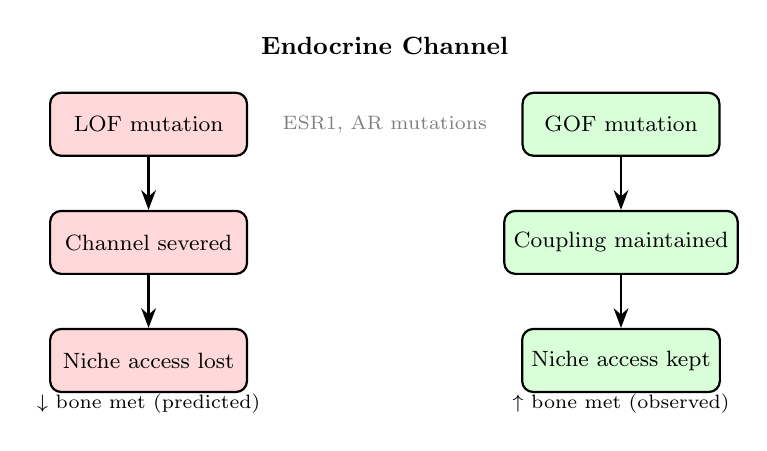
\begin{tikzpicture}[
    box/.style={rectangle, draw=black, thick, rounded corners,
                minimum width=25mm, minimum height=8mm,
                font=\footnotesize},
    lof/.style={box, fill=red!15},
    gof/.style={box, fill=green!15},
    arr/.style={-{Stealth[length=2.5mm]}, thick},
]

% LOF path
\node[lof] (lof) at (-3,2) {LOF mutation};
\node[lof] (sever) at (-3,0.5) {Channel severed};
\node[lof] (lost) at (-3,-1) {Niche access lost};
\node[anchor=south, font=\scriptsize] at (-3,-1.8)
  {$\downarrow$ bone met (predicted)};
\draw[arr] (lof) -- (sever);
\draw[arr] (sever) -- (lost);

% GOF path
\node[gof] (gof) at (3,2) {GOF mutation};
\node[gof] (maintain) at (3,0.5) {Coupling maintained};
\node[gof] (kept) at (3,-1) {Niche access kept};
\node[anchor=south, font=\scriptsize] at (3,-1.8)
  {$\uparrow$ bone met (observed)};
\draw[arr] (gof) -- (maintain);
\draw[arr] (maintain) -- (kept);

% Label
\node[font=\small\bfseries] at (0,3) {Endocrine Channel};
\node[font=\scriptsize, text=gray] at (0,2)
  {ESR1, AR mutations};

\end{tikzpicture}
\caption{GOF vs.\ LOF in the endocrine channel. LOF severs
coupling and should reduce niche-specific tropism. GOF maintains
coupling under therapeutic pressure and preserves tropism. The
endocrine data show GOF: bone metastasis increases, not decreases.
The escalation framework must distinguish severance from resistance.}
\label{fig:gof-lof}
\end{figure}

The data at the single-gene level: prostate cancer AR-mutant
patients, 76.7\% bone metastasis versus 51.4\% AR-wildtype
($p < 10^{-5}$). Breast cancer ESR1/GATA3/FOXA1-mutant, 57.7\%
bone metastasis versus 46.2\% wildtype ($p < 10^{-6}$).

% ------------------------------------------------------------------
\section{Discussion}
\label{sec:discussion}
% ------------------------------------------------------------------

The escalation prediction from Paper~3 holds in cancer, but
the result is sharper than the original prediction. The na\"ive
expectation (connectivity monotonically predicts worse survival)
holds only when bottleneck genes are included. Remove them and
the signal reverses: connectivity becomes protective.

This is the strongest result in the paper because it is
\emph{not} what we initially predicted. We predicted a
continuous gradient. The data revealed two populations with
opposite responses to connectivity. The revised prediction
(bottleneck = harmful, compensation = protective) follows from
the escalation architecture: bottlenecks are irreplaceable paths
whose disruption cascades; compensated nodes have alternative
paths whose redundancy absorbs disruption.

The DDR null result is not a failure of the prediction. It is a
\emph{success}: DDR's parallel architecture means no single gene
is a true bottleneck, so the compensatory (protective) effect of
connectivity dominates.

The BRCA1/BRCA2 case study shows escalation within a single
channel. Same pathway. Different graph position. Different disease.
The hub mutation (BRCA1) produces more aggressive phenotype, more
cross-channel co-mutation (TP53), and different metastatic pattern.
The leaf mutation (BRCA2) is contained. RAD51C confirms: leaf
position, leaf phenotype.

The endocrine GOF finding is the most important result in this
paper, because it is where the data corrected the theory. The
original escalation framework treats any mutation as potential
severance. The endocrine tropism data show that GOF mutations
maintain coupling, not sever it. The framework must distinguish:

\begin{itemize}
\item \textbf{Severance (LOF):} disruption propagates downward,
channel function lost, niche access removed.
\item \textbf{Resistance (GOF):} coupling maintained under
therapeutic pressure, niche access preserved or intensified.
\end{itemize}

This distinction was forced by the data, not fitted to it.

\subsection{What remains to be done}

\begin{enumerate}
\item \textbf{Cancer-type stratification.} The main analysis does
not control for cancer type. TP53 is enriched in aggressive
cancers. The multivariate model should include cancer type as a
covariate to confirm the bottleneck/compensation finding is not
confounded by cancer-type composition.
\item \textbf{Formal bottleneck identification.} Replace ad hoc
``top-$N$'' classification with graph-theoretic bottleneck
detection. Betweenness centrality provides a continuous metric;
the survival data suggest a natural threshold separating the two
populations. Identify this threshold from the data.
\item \textbf{Interaction model.} Fit connectivity $\times$
bottleneck status as an explicit interaction term. The prediction
is a significant crossover interaction: positive coefficient for
connectivity at bottlenecks, negative at compensated nodes.
\item \textbf{Replication in TCGA.} Confirm the two-population
result in an independent (non-MSK) dataset with different panel
composition.
\end{enumerate}

% ------------------------------------------------------------------
\section{Conclusion}
\label{sec:conclusion}
% ------------------------------------------------------------------

Disruption in cancer is not a monotonic function of connectivity.
The graph has two populations: bottleneck genes whose disruption is
catastrophic, and compensated genes whose connectivity is
protective. Connectivity predicts survival ($C = 0.54$), but
removing TP53 and KRAS reverses the signal ($C = 0.48$). Binary
bottleneck classification survives exclusion (HR\,$=$\,1.17,
$p < 10^{-5}$).

This is not what we initially predicted. We predicted a continuous
gradient. The data revealed something sharper: the graph has two
architectural roles, and connectivity operates in opposite
directions depending on which role a gene occupies. The escalation
framework from Paper~3 explains both directions. Bottlenecks are
irreplaceable paths; their disruption cascades. Compensated nodes
have redundant paths; their connectivity absorbs disruption.

The GOF/LOF distinction is the second necessary refinement: not all
mutations are severance. Some maintain coupling under pressure.
The escalation framework must track both direction (LOF vs.\ GOF)
and position (bottleneck vs.\ compensated).

\section*{Acknowledgments}

The author used Claude (Anthropic) for drafting assistance,
literature review, and \LaTeX{} preparation. All theoretical
content, analyses, and arguments are the author's own.

\bibliographystyle{plain}
\begin{thebibliography}{99}

\bibitem{McCarthy2026a}
P.~D. McCarthy.
\newblock Graph structure is necessary for information preservation under
  bounded context.
\newblock Manuscript, 2026.

\bibitem{McCarthy2026c}
P.~D. McCarthy.
\newblock Convergence of control architectures to escalation under bounded
  context.
\newblock Manuscript, 2026.

\bibitem{McCarthy2026e}
P.~D. McCarthy.
\newblock Coupling-channel count predicts cancer survival better than mutation
  count.
\newblock Manuscript, 2026.

\bibitem{Zehir2017}
A.~Zehir, R.~Benayed, R.~H. Shah, A.~Syed, S.~Middha,
  H.~R. Kim, P.~Srinivasan, J.~Gao, D.~Chakravarty,
  S.~M. Devlin, and others.
\newblock Mutational landscape of metastatic cancer revealed from
  prospective clinical sequencing of 10,000 patients.
\newblock \emph{Nature Medicine}, 23(6):703--713, 2017.

\bibitem{Nguyen2022}
B.~Nguyen et~al.
\newblock Genomic characterization of metastatic patterns from
  prospective clinical sequencing of 25,000 patients.
\newblock \emph{Cell}, 185(3):563--575, 2022.

\bibitem{Bandlamudi2024}
C.~Bandlamudi, J.~J.~Harding, A.~Zehir, and others.
\newblock Clinical genomic profiling of 50,000 patients:
  Experience from the {MSK-IMPACT} clinical sequencing cohort.
\newblock \emph{Cancer Cell}, 2024.

\bibitem{Szklarczyk2023}
D.~Szklarczyk et~al.
\newblock The {STRING} database in 2023.
\newblock \emph{Nucleic Acids Research}, 51(D1):D483--D489, 2023.

\bibitem{Jassal2020}
B.~Jassal et~al.
\newblock The {R}eactome pathway knowledgebase.
\newblock \emph{Nucleic Acids Research}, 48(D1):D498--D503, 2020.

\bibitem{Hanahan2011}
D.~Hanahan and R.~A. Weinberg.
\newblock Hallmarks of cancer: The next generation.
\newblock \emph{Cell}, 144(5):646--674, 2011.

\end{thebibliography}

\end{document}
